\section{Physicochemical and Toxicological Interfaces of Pristine Lunar Regolith}
\label{sec:toxicology}

\subsection{Nanophase Iron and Abiotic Reactive Oxygen Species Generation}
\label{subsec:npfe_ros}

The Moon's hyper-vacuum environment and absence of a global dipolar magnetosphere expose surface minerals to unattenuated space weathering\cite{paul2022plants,ming1989lunar,hendrix2024reactivity,turci2015mechanistic}. Solar wind proton bombardment reduces ferrous silicates, while episodic micrometeorite impacts induce localized shock melting and vapor-phase condensation\cite{ming1989lunar,liu2013microwave}. These energetic processes generate nanophase metallic iron ($\mathrm{npFe}^0$), consisting of zero-valent iron blebs ($1\text{--}100\,\mathrm{nm}$ in diameter) embedded within mineral rims and dispersed throughout the amorphous silicate matrices of agglutinitic glasses\cite{paul2022plants,ming1989lunar,lytvynenko2021lunar}.

When pristine regolith or reduced lunar simulants contact oxygenated aqueous solutions within a pressurized habitat, these surface-accessible metallic blebs trigger abiotic oxidation cascades\cite{ming1989lunar,hendrix2024reactivity,turci2015mechanistic}. Solvated divalent ferrous ions ($\mathrm{Fe}^{2+}$) dissolve from mineral interfaces in the presence of dissolved oxygen, initiating modified Fenton-like catalytic cycles\cite{ming1989lunar,hendrix2024reactivity,turci2015mechanistic}:
\begin{equation}
    \mathrm{Fe}^0 + \mathrm{O}_2 + 2\mathrm{H}^+ \longrightarrow \mathrm{Fe}^{2+} + \mathrm{H}_2\mathrm{O}_2
    \label{eq:fe0_dissolution}
\end{equation}
Subsequent electron transfer between the released ferrous iron and ambient oxidants drives the generation of hydroxyl free radicals ($\cdot\mathrm{OH}$) and superoxide radical anions ($\mathrm{O}_2^{\cdot-}$):
\begin{align}
    \mathrm{Fe}^{2+} + \mathrm{H}_2\mathrm{O}_2 &\longrightarrow \mathrm{Fe}^{3+} + \cdot\mathrm{OH} + \mathrm{OH}^- \label{eq:fenton_reaction} \\
    \mathrm{Fe}^{2+} + \mathrm{O}_2 &\longleftrightarrow \mathrm{Fe}^{3+} + \mathrm{O}_2^{\cdot-} \label{eq:superoxide_reaction}
\end{align}

Electron paramagnetic resonance (EPR) spectroscopy with spin-trapping adducts, alongside chemical terephthalate hydroxylation assays, confirms that reduced lunar materials generate hydroxyl radical concentrations 5-fold to 100-fold higher than unreduced terrestrial basaltic analogs\cite{hendrix2024reactivity,turci2015mechanistic,wallace2022assessment}. Furthermore, mechanical impact crushing on the airless lunar surface cleaves covalent bonds in silicates, plagioclase, and pyroxenes without atmospheric passivating agents, leaving surface dangling bonds such as broken silicon radicals ($\equiv\!\mathrm{Si}\cdot$) and silicon-peroxyl radicals ($\equiv\!\mathrm{Si}-\mathrm{O}\cdot$)\cite{turci2015mechanistic,schoonen2020hydroxyl}. Upon hydration, these radicals homolytically split water molecules, generating sustained bursts of oxidizing species\cite{schoonen2020hydroxyl,sperl2017influence}. Direct contact with this abiotic interface subjects plant root cell membranes to rapid lipid peroxidation, disrupting transmembrane electrochemical gradients, destroying transport proteins, and inducing root apical growth arrest\cite{ming1989lunar,turci2015mechanistic}.

\subsection{Transcriptomic Reprogramming, Genomic Lesions, and Morphological Impedance}
\label{subsec:transcriptomics_genomics}

The biological consequences of these reactive interfaces were demonstrated empirically by Paul et al.\cite{paul2022plants} using authentic lunar soils returned by Apollo 11, 12, and 17. Seeds of \textit{Arabidopsis thaliana} germinated uniformly across Apollo regolith samples and volcanic controls; however, post-germination ontogeny diverged sharply\cite{paul2022plants}. Seedlings cultivated directly in Apollo regoliths exhibited severe stress phenotypes, including arrested primary root elongation, stunted rosette expansion, retarded leaf development, and dark purple pigmentation driven by anthocyanin hyperaccumulation\cite{paul2022plants,paul2022biological}.

High-throughput RNA sequencing revealed that plants grown in raw lunar regolith execute a systemic transcriptomic reprogramming, shifting metabolic resources from vegetative biomass accumulation to protective defense cascades\cite{paul2022plants,lytvynenko2021lunar}. Differentially expressed genes are dominated by pathways associated with heavy metal toxicity, osmotic shock, and oxidative burst defense\cite{paul2022plants,lytvynenko2021lunar}. Plants significantly upregulate transcripts encoding glutathione S-transferases (GSTs), class III secretory cell-wall peroxidases, heat shock transcription factors, and antioxidant enzymes\cite{paul2022plants,lytvynenko2021lunar}. Concurrently, signaling cascades mediated by jasmonic acid (JA) and abscisic acid (ABA) are chronically induced, repressing cell-wall loosening and cellular expansion\cite{paul2022plants,ming1989lunar}. The magnitude of transcriptomic stress correlates positively with regolith maturity, quantified by the ferromagnetic resonance (FMR) maturity index ($I_s/\mathrm{FeO}$)\cite{paul2022plants,paul2022biological,morris1976surface}. Mature regoliths (e.g., Apollo 11 sample 10084 and Apollo 17 sample 70051), possessing high agglutinitic glass and $\mathrm{npFe}^0$ contents, trigger significantly more intense stress responses than immature sub-surface samples (e.g., Apollo 12 sample 12070)\cite{paul2022plants,paul2022biological}.

Beyond immediate physiological stress, continuous root exposure to raw regolith compromises long-term genomic stability\cite{barbero2024telomere,shippen2019telomere}. Multi-generational cultivation experiments utilizing regolith simulants demonstrate progressive accumulation of 8-oxoguanine (8-oxoG) DNA lesions induced by oxidative stress\cite{barbero2024telomere}. Because chromosomal telomeres contain repetitive guanine-rich motifs, they act as primary targets for oxidative damage\cite{barbero2024telomere,min2023protection}. In regolith simulant environments, telomerase catalytic activity becomes uncoupled from telomere length maintenance, culminating in accelerated telomere shortening, genome instability, and loss of multi-generational fitness\cite{ming1989lunar,barbero2024telomere}.

These biochemical challenges are compounded by particle morphometry\cite{paul2022plants,ming1989lunar,fackrell2024mechanical}. Lacking atmospheric tumbling or aqueous rounding regimes, lunar particles retain razor-sharp edges with extreme aspect ratios\cite{paul2022plants,ming1989lunar,fackrell2024mechanical}. As expanding root tips penetrate these interlocking angular grains, the abrasive surfaces micro-shear the root cap, strip mucilage-secreting border cells, and tear epidermal tissues\cite{ming1989lunar,hendrix2024reactivity}. Plants must continuously expend metabolic energy repairing damaged epidermal barriers, resulting in a systemic physiological penalty that curtails edible crop yields\cite{ming1989lunar,fackrell2024mechanical}.

\begin{figure}[t!]
    \centering
    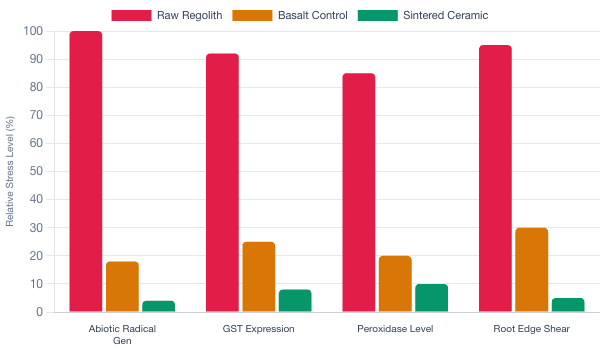
\includegraphics[width=0.92\textwidth]{figures/fig1_toxicity_passivation.png}
    \caption{\textbf{Physicochemical and toxicological interfaces of raw versus sintered lunar regolith.} (\textbf{a}) Raw lunar regolith contains reactive nanophase metallic iron ($\mathrm{npFe}^0$), broken silicate dangling bonds, and razor-sharp mineral shards that generate chronic oxidative stress via modified Fenton reactions ($\mathrm{Fe}^0 \to \mathrm{Fe}^{2+} \to \cdot\mathrm{OH}, \mathrm{O}_2^{\cdot-}$), damaging plant root membranes and inducing 8-oxoG genomic lesions. (\textbf{b}) Thermal sintering above $1050^\circ\mathrm{C}$ passivates these hazards by oxidizing $\mathrm{npFe}^0$ into stable augite and olivine crystal matrices, rounding abrasive grain boundaries, and restoring plant transcriptomic homeostasis.}
    \label{fig:toxicity_passivation}
\end{figure}

\begin{table}[t!]
\small
\centering
\caption{\textbf{Comparative physicochemical, toxicological, and agronomic properties of raw lunar regolith versus sintered regolith ceramics.}}
\label{tab:toxicity_comparison}
\begin{tabularx}{\textwidth}{lXX}
\toprule
\textbf{Parameter / Property} & \textbf{Raw Lunar Regolith (Direct Cultivation)} & \textbf{Sintered Regolith Ceramic (Engineered Substrate)} \\
\midrule
Nanophase Metallic Iron ($\mathrm{npFe}^0$) & Surface-accessible blebs across grain rims ($1\text{--}100\,\mathrm{nm}$)\cite{paul2022plants,ming1989lunar,lytvynenko2021lunar} & Oxidized and incorporated into stable crystalline silicates\cite{ming1989lunar,taylor2005microwave} \\
\addlinespace
Aqueous ROS Generation Potential & High; sustained $\cdot\mathrm{OH}$ and $\mathrm{O}_2^{\cdot-}$ generation via Fenton pathways\cite{paul2022plants,hendrix2024reactivity,turci2015mechanistic} & Negligible; passivated, hydrothermally inert interface\cite{ming1989lunar,turci2015mechanistic,sperl2017influence} \\
\addlinespace
Grain / Pore Morphometry & Highly angular, sharp, micro-shearing shards\cite{ming1989lunar,hendrix2024reactivity,fackrell2024mechanical} & Rounded, smooth, consolidated neck boundaries\cite{ming1989lunar,xi2026multiphysics,goulas2017process} \\
\addlinespace
Plant Transcriptomic Profile & Chronic upregulation of GSTs, peroxidases, JA, and ABA stress pathways\cite{paul2022plants,paul2022biological,lytvynenko2021lunar} & Homeostatic baseline; standard vegetative and reproductive allocation\cite{paul2022plants,ming1989lunar} \\
\addlinespace
Chromosomal \& Telomeric Integrity & Elevated 8-oxoG lesions, accelerated telomere erosion, fitness decline\cite{barbero2024telomere,shippen2019telomere,min2023protection} & Protected genome; absence of mineral-derived radical stress\cite{ming1989lunar,barbero2024telomere} \\
\addlinespace
Interfacial Contact Angle & Initially hydrophobic; prone to liquid beading and bypass channeling\cite{paul2022plants,paul2022biological,steinberg2007fluid} & Tailored hydrophilic wettability; continuous capillary wicking\cite{ming1989lunar,heinse2007porous} \\
\addlinespace
Aqueous Solution Chemistry & Uncontrolled dissolution; alkaline spikes ($\mathrm{pH}\;9.0\text{--}11.0$), P-fixation\cite{ming1989lunar,hendrix2024reactivity,wamelink2024struvite} & Stable $\mathrm{pH}$ control ($\mathrm{pH}\;5.8\text{--}6.2$); predictable nutrient stoichiometry\cite{ming1989lunar} \\
\bottomrule
\end{tabularx}
\end{table}
